\section{Floating Platform}
The floating platform, depicted in
\cref{fig:floatingPlatform}, is the main structure of the built vehicle.
It is a baffle of glulam wood, with two pieces of XPS cell foam as
pontoons, where all the components are attached. It can keep a mass of
around 20~kg above water with margins.

In the middle of the platform two symmetrical holes with fittings was
been made, in which the RBR modules can be attached or detached. In the front of the platform a large rounded bumper helps with deflection of head on collisions. It also creates a distance between the platform and
any side obstacles, which helps maneuvering in tight spots and sharp corners. In the
middle of the platform the majority of the electronics has been placed. The electronics and the RBR modules have acrylic
protection covers, protecting the equipment from small splashes of water and rain.

\begin{figure}[h]
   \centering
   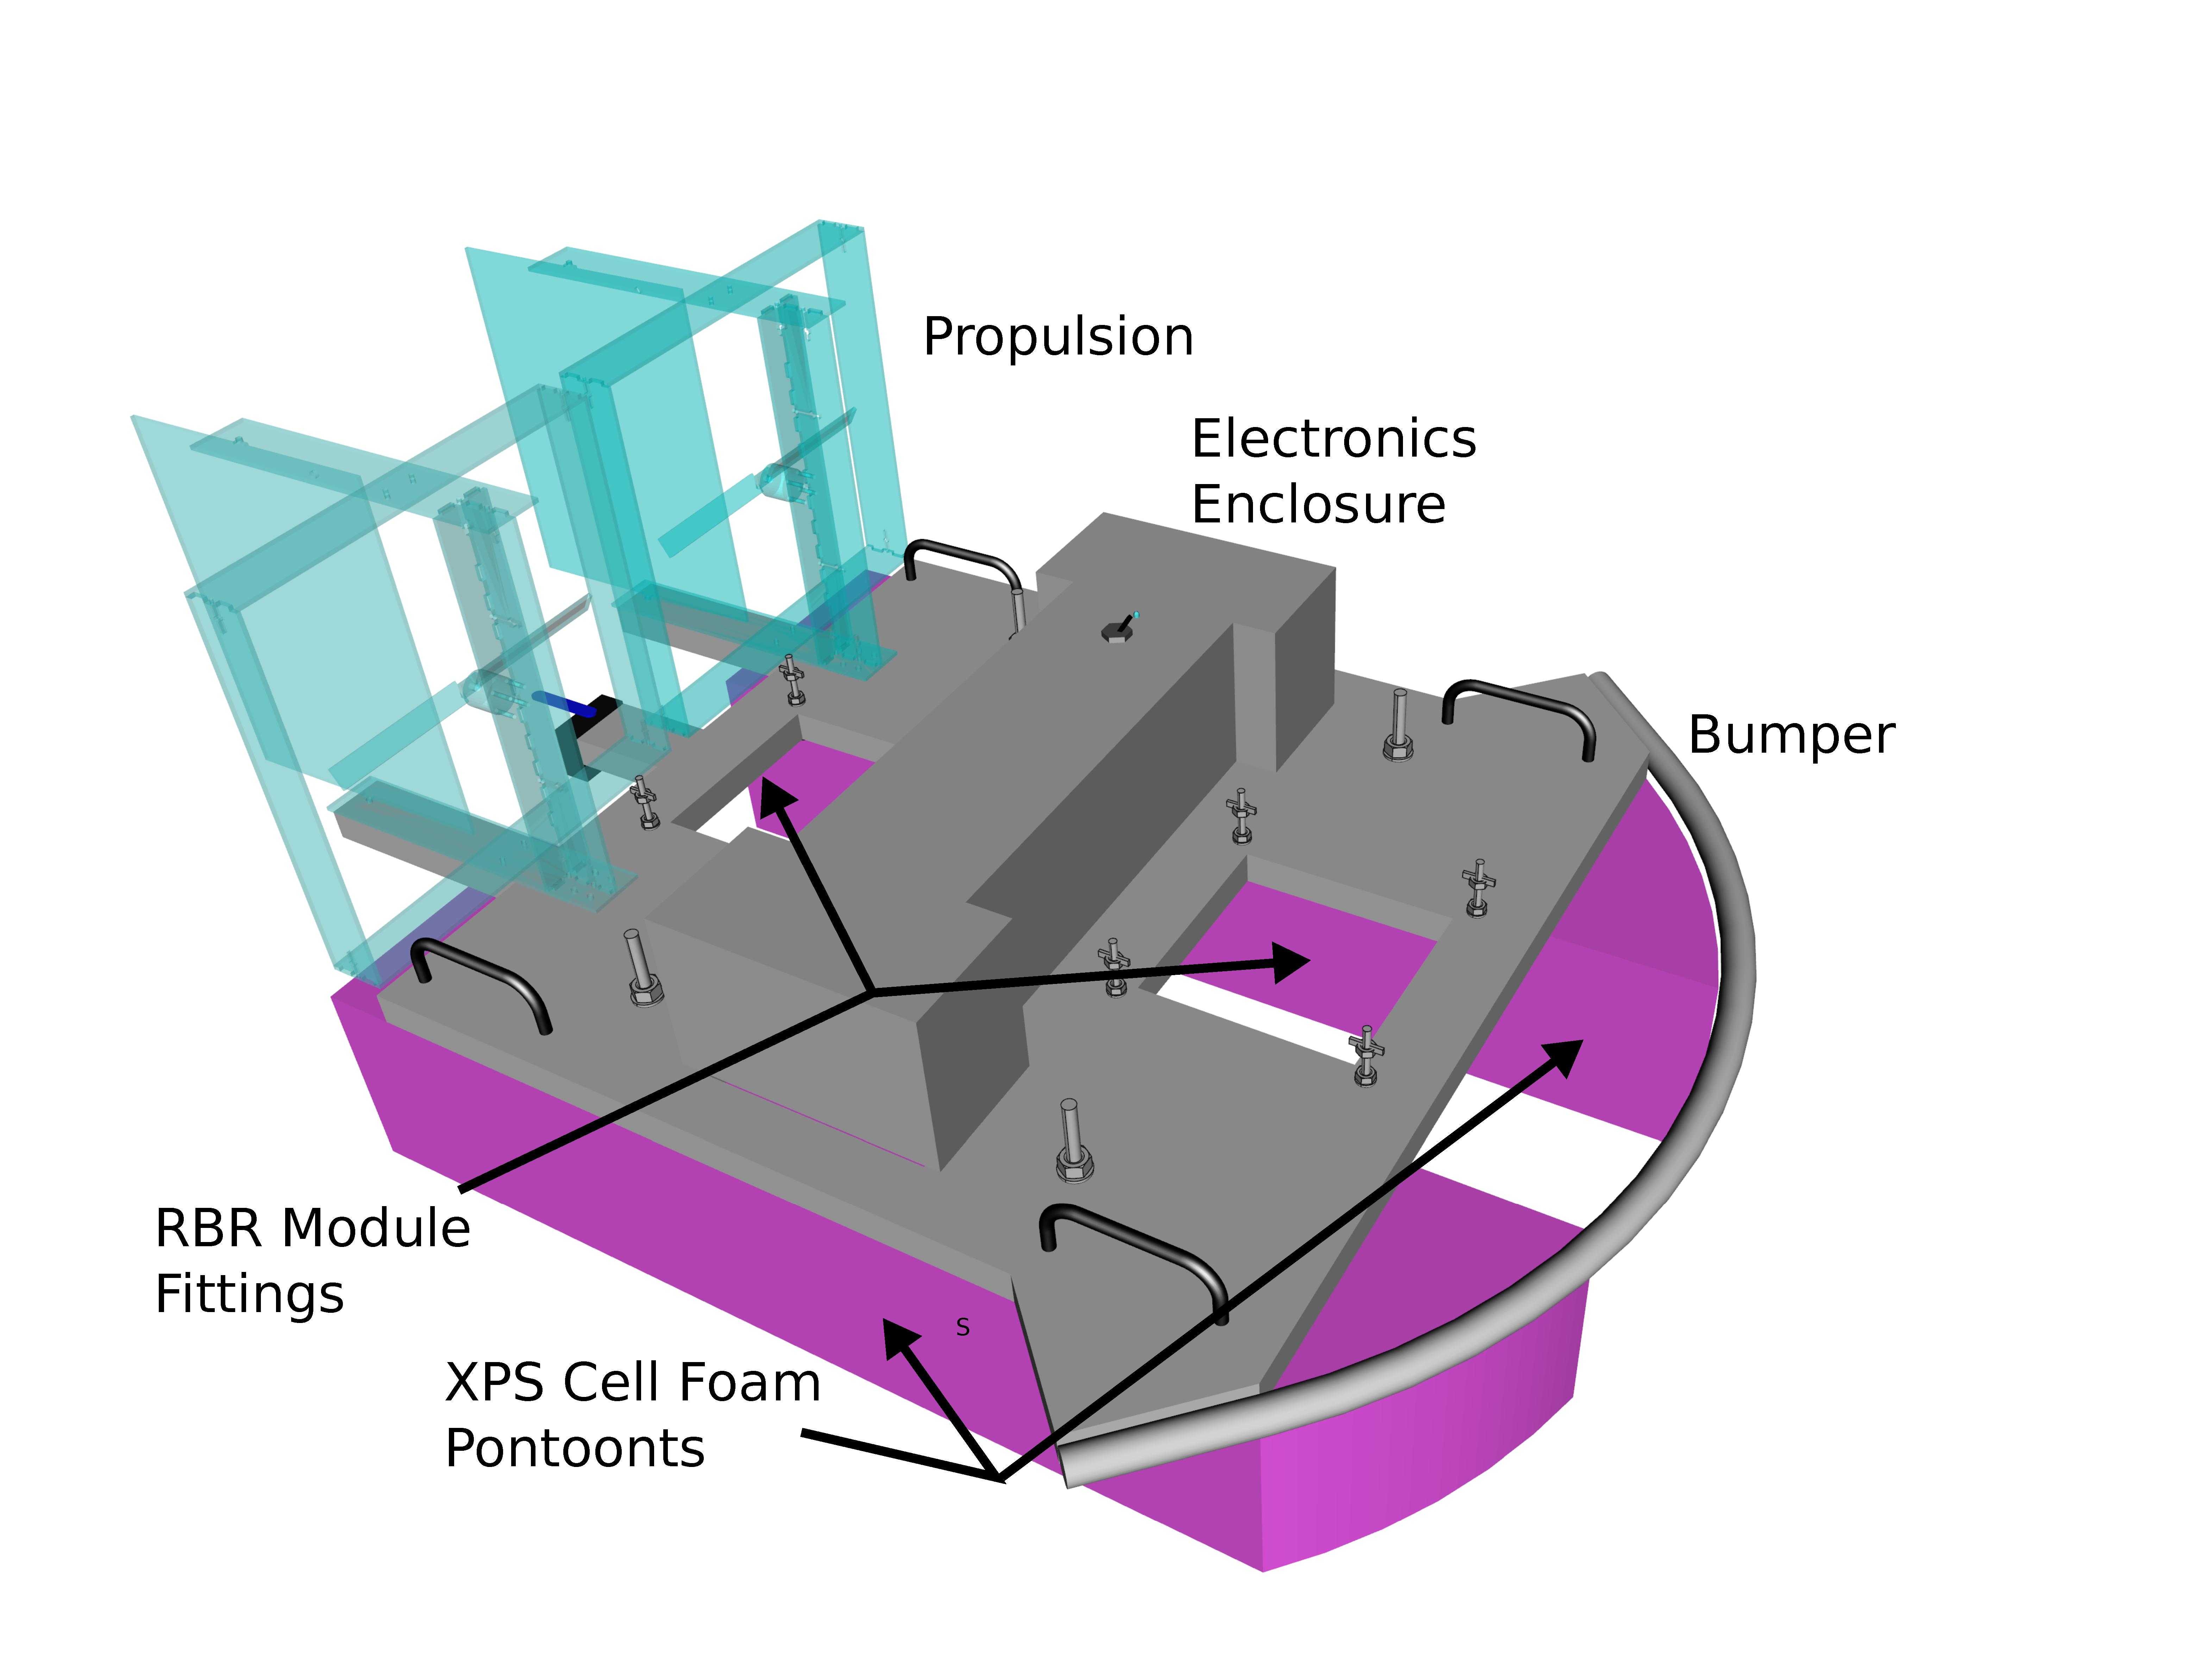
\includegraphics[width=.75\textwidth]{platformWithNotes.eps}
   \caption{The floating platform without the RBR modules installed.}
   \label{fig:floatingPlatform}
\end{figure}

\subsection{RBR module}
The RBR module, seen in fig. \ref{fig:rbr-module} consist of two baffles, separated by three adjustable threaded
rods. The upper mounted baffle is constructed with a modified hand-held screwdriver. The lower mounted
baffle has a PTFE shaft guide mounted for a RBR axle. A shaft can then be driven through the shaft guide and be attached to the screwdriver, in order to drive the RBRs under water. The lower mounted baffle has an
additional baffle which goes down into the water just above where a mounted RBR
will be situated. This baffle prevents the formation of large vortices above the RBR. 

\begin{figure}[H]
  \centering
  \textbf{RBR module}
  \par\medskip
  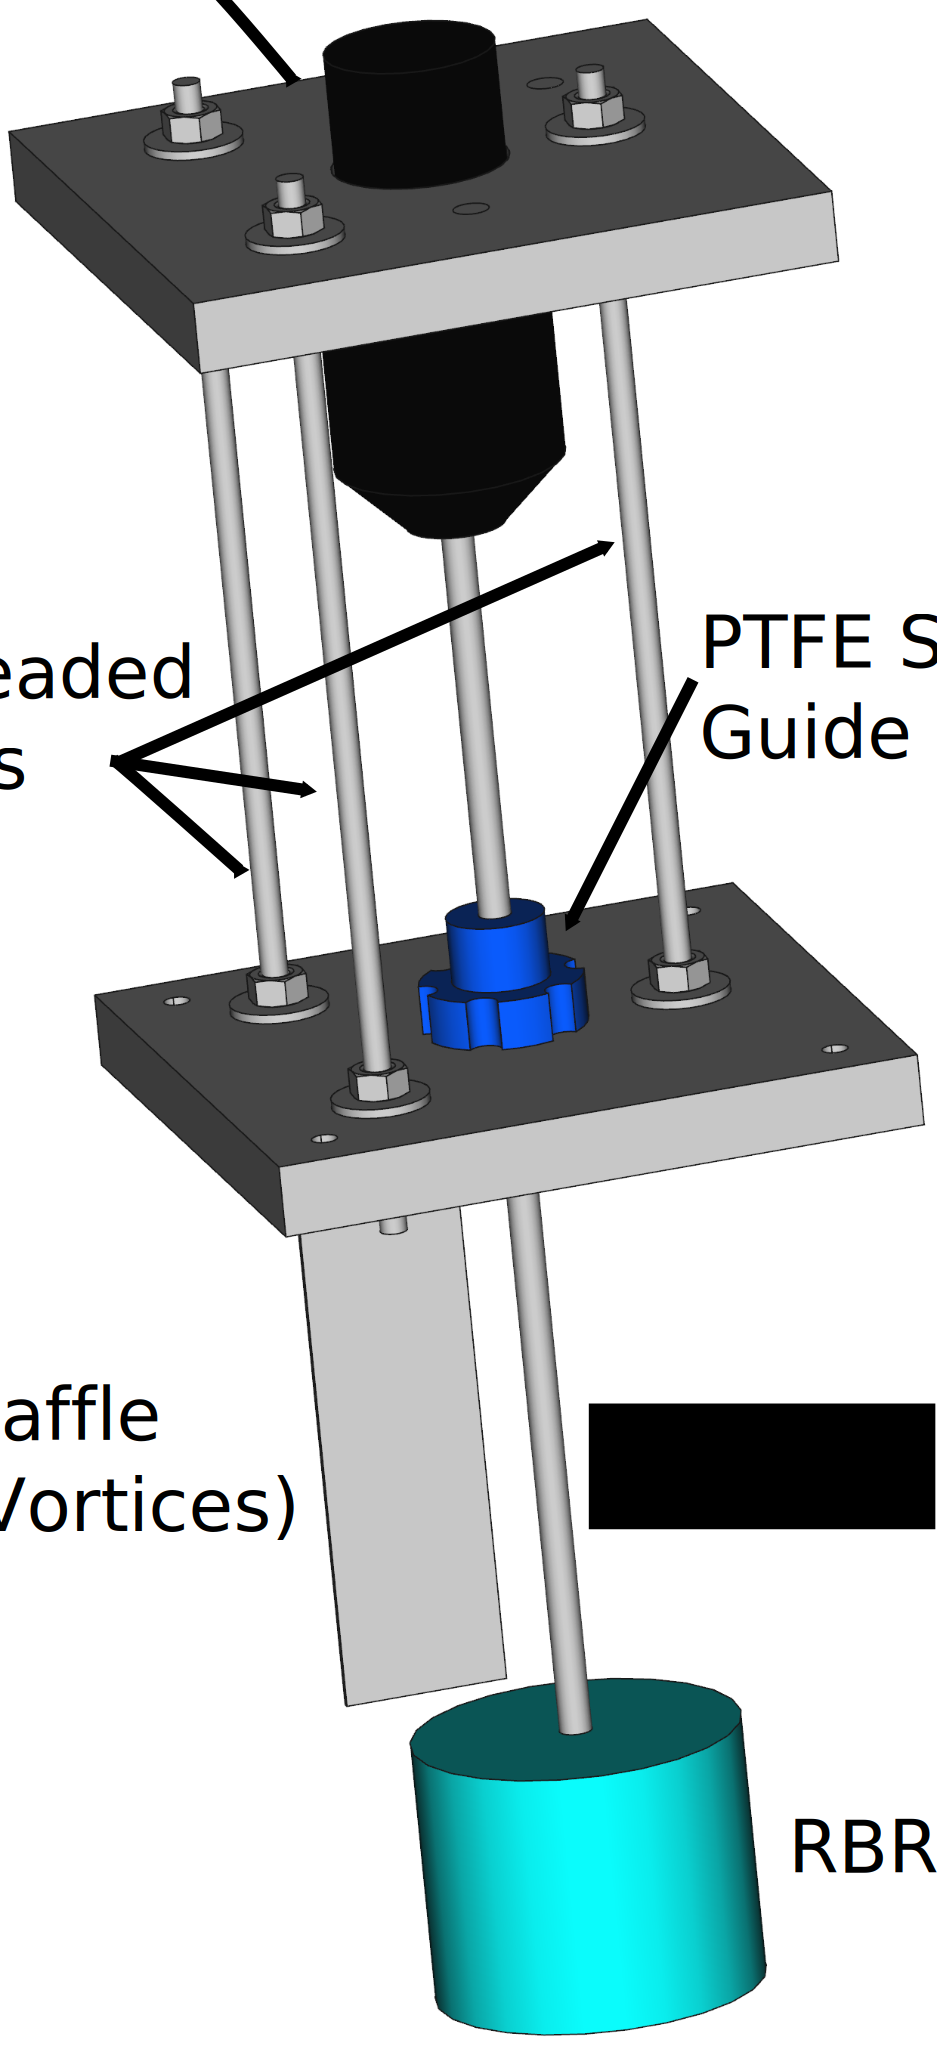
\includegraphics[width=0.5\textwidth]{RBR-moduleWithNotes}
  \caption{A RBR module with a drive assembly mounted at the top baffle,
    which in turn is mounted with adjustable threaded rods to the lower baffle. This houses the shaft guide for the RBR axle. The lower baffle mounts to the
    top of the platform, and on the RBR modules underside sits a wave baffle.}\label{fig:rbr-module}
\end{figure}

The upper baffle can be height adjusted, in order to easily calibrate the desired depth of the RBR. It is ideal to have the RBR distanced from the water surface. It is preferred to have it at a lower level than the bottom of the pontoons to prevent air reaching the RBR. 

The speed of the RBRs can be controlled remotely. The rotational speed interval of the RBR ranges from 0 to 600 rpm, where 500~rpm is ideal.


The RBR modules can be attached to the intended slots on the platform. The modules should be oriented such that the vertical baffle is parallel to the travel direction to minimize the vehicles water friction. Fly nuts are used to hold the modules in the slots. 

\subsection{Propulsion}
The propulsion is made from air-propellers, installed in an acrylic plastic protection housing. Acrylic plastic rudders were installed in front of the propellers, these are controlled through a single servo located at the back of the platform. The layout of the propulsion mechanism is shown in \cref{fig:propellerWithNotes}.

\begin{figure}[h]
   \centering
   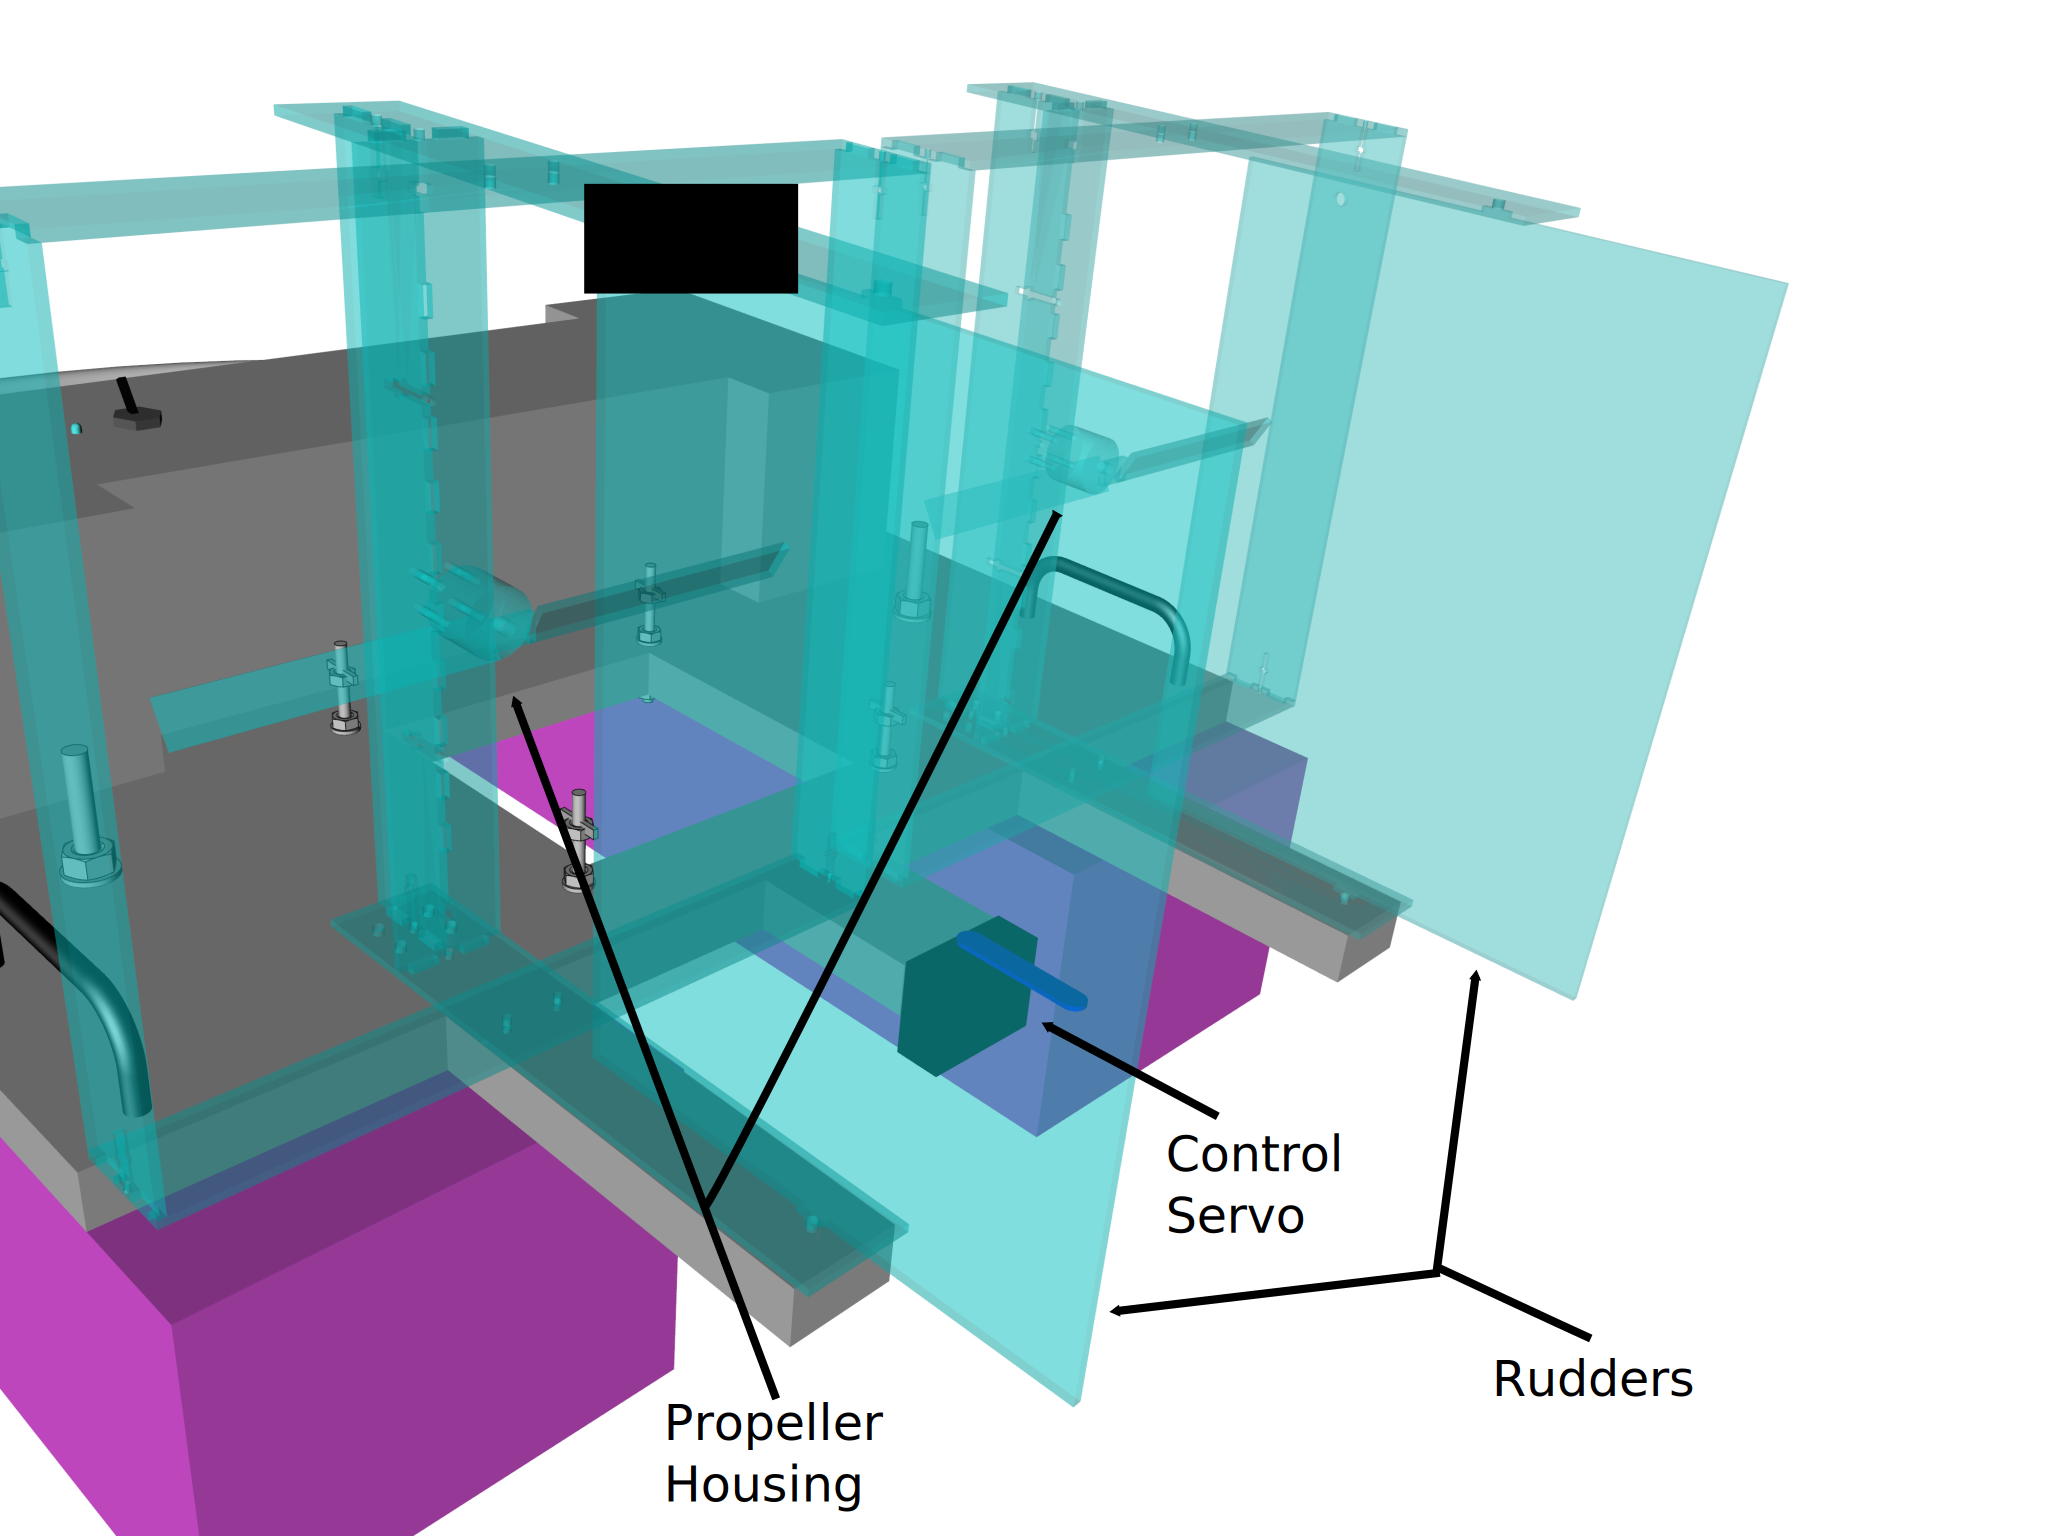
\includegraphics[width=.75\textwidth]{propellerWithNotes}
   \caption{The propulsion construction.}
   \label{fig:propellerWithNotes}
\end{figure}

\subsection{Water protection}

An acrylic protection cover were manufactured in order to protect the batteries, the engine control units, and other electronic equipment. Two separate acrylic covers were also constructed to protect the drive assemblies of the RBR modules. The covers do not protect the equipment from submersion, only from small splashes or rain. To install the covers, just place them over the RBR modules. The cover for the electronics is held in place with one screw on either side of the electronic enclosure.

\subsection{Transportation}

To ease transportation, the weight of the platform can be reduced. This is done by first removing the protective covers, followed by disconnecting the power cables connected to the batteries and RBR drive assembly. It is then possible to remove the batteries and RBR modules from the platform. During transport care needs to be taken such that the propulsion mounts are not damaged, as these parts are fragile.